\documentclass[11pt]{article}
\usepackage{amsgen,amsmath,amstext,amsbsy,amsopn,amssymb}
%\usepackage[dvips]{graphicx,color}
\usepackage{graphicx,color}
\usepackage{graphicx,color,bm}
\usepackage{epsfig}
\usepackage{enumerate}
\usepackage{float}

%\setlength{\oddsidemargin}{0.1 in} \setlength{\evensidemargin}{-0.1
%in} \setlength{\topmargin}{-0.6 in} \setlength{\textwidth}{6.5 in}
%\setlength{\textheight}{8.5 in} \setlength{\headsep}{0.75 in}
%\setlength{\parindent}{0 in} \setlength{\parskip}{0.1 in}

\textwidth 6.3in \textheight 8.8in \topmargin -0.5truein
\oddsidemargin .15truein
\parskip .1in
\renewcommand{\baselinestretch}{1.53}  % double spaced


\newcommand{\homework}[6]{
	\pagestyle{myheadings}
	\thispagestyle{plain}
	\newpage
	\setcounter{page}{1}
	\noindent
	\begin{center}
		\framebox{
			\vbox{\vspace{2mm}
				\hbox to 6.28in { {\bf Math531:~Regression - I  \hfill} }
				\vspace{6mm}
				\hbox to 6.28in { {\Large \hfill #1 (#2)  \hfill} }
				\vspace{6mm}
				\hbox to 6.28in { {\it Instructor: #3 \hfill} }
				\hbox to 6.28in { {\it Office hours: #4  \hfill #6}}
				\vspace{2mm}}
		}
	\end{center}
	\markboth{#1}{#1}
	\vspace*{4mm}
}

% ----------------------- MATH -------------------------
\def\av{\boldsymbol a}
\def\bv{\boldsymbol b}
\def\cv{\boldsymbol c}
\def\dv{\boldsymbol d}
\def\ev{\boldsymbol e}
\def\fv{\boldsymbol f}
\def\gv{\boldsymbol g}
\def\hv{\boldsymbol h}
\def\iv{\boldsymbol i}
\def\gv{\boldsymbol j}
\def\kv{\boldsymbol k}
\def\lv{\boldsymbol l}
\def\mv{\boldsymbol m}
\def\nv{\boldsymbol n}
\def\ov{\boldsymbol o}
\def\pv{\boldsymbol p}
\def\qv{\boldsymbol q}
\def\rv{\boldsymbol r}
\def\sv{\boldsymbol s}
\def\tv{\boldsymbol t}
\def\uv{\boldsymbol u}
\def\vv{\boldsymbol v}
\def\wv{\boldsymbol w}
\def\xv{\boldsymbol x}
\def\yv{\boldsymbol y}
\def\zv{\boldsymbol z}
\def\Av{\boldsymbol A}
\def\Bv{\boldsymbol B}
\def\Cv{\boldsymbol C}
\def\Dv{\boldsymbol D}
\def\Ev{\boldsymbol E}
\def\Fv{\boldsymbol F}
\def\Gv{\boldsymbol G}
\def\Hv{\boldsymbol H}
\def\Iv{\boldsymbol I}
\def\Gv{\boldsymbol J}
\def\Kv{\boldsymbol K}
\def\Lv{\boldsymbol L}
\def\Mv{\boldsymbol M}
\def\Nv{\boldsymbol N}
\def\Ov{\boldsymbol O}
\def\Pv{\boldsymbol P}
\def\Qv{\boldsymbol Q}
\def\Rv{\boldsymbol R}
\def\Sv{\boldsymbol S}
\def\Tv{\boldsymbol T}
\def\Uv{\boldsymbol U}
\def\Vv{\boldsymbol V}
\def\Wv{\boldsymbol W}
\def\Xv{\boldsymbol X}
\def\Yv{\boldsymbol Y}
\def\Zv{\boldsymbol Z}
\def\Abf{\mathbf A}
\def\Bbf{\mathbf B}
\def\Cbf{\mathbf C}
\def\Dbf{\mathbf D}
\def\Ebf{\mathbf E}
\def\Fbf{\mathbf F}
\def\Gbf{\mathbf G}
\def\Hbf{\mathbf H}
\def\Ibf{\mathbf I}
\def\Gbf{\mathbf J}
\def\Kbf{\mathbf K}
\def\Lbf{\mathbf L}
\def\Mbf{\mathbf M}
\def\Nbf{\mathbf N}
\def\Obf{\mathbf O}
\def\Pbf{\mathbf P}
\def\Qbf{\mathbf Q}
\def\Rbf{\mathbf R}
\def\Sbf{\mathbf S}
\def\Tbf{\mathbf T}
\def\Ubf{\mathbf U}
\def\Vbf{\mathbf V}
\def\Wbf{\mathbf W}
\def\Xbf{\mathbf X}
\def\Ybf{\mathbf Y}
\def\Zbf{\mathbf Z}
\def\Am{\mathrm A}
\def\Bm{\mathrm B}
\def\Cm{\mathrm C}
\def\Dm{\mathrm D}
\def\Em{\mathrm E}
\def\Fm{\mathrm F}
\def\Gm{\mathrm G}
\def\Hm{\mathrm H}
\def\Im{\mathrm I}
\def\Gm{\mathrm J}
\def\Km{\mathrm K}
\def\Lm{\mathrm L}
\def\Mm{\mathrm M}
\def\Nm{\mathrm N}
\def\Om{\mathrm O}
\def\Pm{\mathrm P}
\def\Qm{\mathrm Q}
\def\Rm{\mathrm R}
\def\Sm{\mathrm S}
\def\Tm{\mathrm T}
\def\Um{\mathrm U}
\def\mv{\mathrm V}
\def\Wm{\mathrm W}
\def\Xm{\mathrm X}
\def\Ym{\mathrm Y}
\def\Zm{\mathrm Z}
\newcommand{\Ac}{\mathcal{A}}
\newcommand{\Bc}{\mathcal{B}}
\newcommand{\Cc}{\mathcal{C}}
\newcommand{\Dc}{\mathcal{D}}
\newcommand{\Ec}{\mathcal{E}}
\newcommand{\Fc}{\mathcal{F}}
\newcommand{\Gc}{\mathcal{G}}
\newcommand{\Hc}{\mathcal{H}}
\newcommand{\Ic}{\mathcal{I}}
\newcommand{\Jc}{\mathcal{J}}
\newcommand{\Kc}{\mathcal{K}}
\newcommand{\Lc}{\mathcal{L}}
\newcommand{\Mc}{\mathcal{M}}
\newcommand{\Nc}{\mathcal{N}}
\newcommand{\Oc}{\mathcal{O}}
\newcommand{\Pc}{\mathcal{P}}
\newcommand{\Qc}{\mathcal{Q}}
\newcommand{\Rc}{\mathcal{R}}
\newcommand{\Sc}{\mathcal{S}}
\newcommand{\Tc}{\mathcal{T}}
\newcommand{\Uc}{\mathcal{U}}
\newcommand{\Vc}{\mathcal{V}}
\newcommand{\Wc}{\mathcal{W}}
\newcommand{\Xc}{\mathcal{X}}
\newcommand{\Yc}{\mathcal{Y}}
\newcommand{\Zc}{\mathcal{Z}}
\newcommand{\alphav}{\mbox{\boldmath{$\alpha$}}}
\newcommand{\betav}{\mbox{\boldmath{$\beta$}}}
\newcommand{\gammav}{\mbox{\boldmath{$\gamma$}}}
\newcommand{\deltav}{\mbox{\boldmath{$\delta$}}}
\newcommand{\epsilonv}{\mbox{\boldmath{$\epsilon$}}}
\newcommand{\zetav}{\mbox{\boldmath$\zeta$}}
\newcommand{\etav}{\mbox{\boldmath{$\eta$}}}
\newcommand{\iotav}{\mbox{\boldmath{$\iota$}}}
\newcommand{\kappav}{\mbox{\boldmath{$\kappa$}}}
\newcommand{\lambdav}{\mbox{\boldmath{$\lambda$}}}
\newcommand{\muv}{\mbox{\boldmath{$\mu$}}}
\newcommand{\nuv}{\mbox{\boldmath{$\nu$}}}
\newcommand{\xiv}{\mbox{\boldmath{$\xi$}}}
\newcommand{\omicronv}{\mbox{\boldmath{$\omicron$}}}
\newcommand{\piv}{\mbox{\boldmath{$\pi$}}}
\newcommand{\rhov}{\mbox{\boldmath{$\rho$}}}
\newcommand{\sigmav}{\mbox{\boldmath{$\sigma$}}}
\newcommand{\tauv}{\mbox{\boldmath{$\tau$}}}
\newcommand{\upsilonv}{\mbox{\boldmath{$\upsilon$}}}
\newcommand{\phiv}{\mbox{\boldmath{$\phi$}}}
\newcommand{\varphiv}{\mbox{\boldmath{$\varphi$}}}
\newcommand{\chiv}{\mbox{\boldmath{$\chi$}}}
\newcommand{\psiv}{\mbox{\boldmath{$\psi$}}}
\newcommand{\omegav}{\mbox{\boldmath{$\omega$}}}
\newcommand{\Sigmav}{\mbox{\boldmath{$\Sigma$}}}
\newcommand{\Lambdav}{\mbox{\boldmath{$\Lambda$}}}
\newcommand{\Deltav}{\mbox{\boldmath{$\Delta$}}}
\newcommand{\Omegav}{\mbox{\boldmath{$\Omega$}}}
\newcommand{\varepsilonv}{\mbox{\boldmath{$\varepsilon$}}}

\newcommand{\eps}{\varepsilon}
\newcommand{\epsv}{\mbox{\boldmath{$\varepsilon$}}}

\def\1v{\mathbf 1}
\def\0v{\mathbf 0}
\def\Id{\mathbf I} % identity matrix
\newcommand{\ind}[1]{\mathbbm{1}_{\left[ {#1} \right] }}
\newcommand{\Ind}[1]{\mathbbm{1}_{\left\{ {#1} \right\} }}
\newcommand\indep{\protect\mathpalette{\protect\independenT}{\perp}}\def\independenT#1#2{\mathrel{\rlap{$#1#2$}\mkern2mu{#1#2}}}
\newcommand{\QED}{\begin{flushright} {\bf QED} \end{flushright}}
\newcommand{\R}{\mathbb R}
\newcommand{\Real}{\mathbb R}
\newcommand{\C}{\mathbb C}
\newcommand{\E}{\mathbb E}
\newcommand{\sgn}{\mathop{\mathrm{sign}}}
\def\Pr{\mathrm P}
\def\pr{\mathrm P}
\newcommand{\Var}{\mathop{\rm Var}}
\newcommand{\var}{\mathop{\rm Var}}
\newcommand{\Cov}{\mathop{\rm Cov}}
\newcommand{\cov}{\mathop{\rm Cov}}
\newcommand{\Corr}{\mathop{\rm Corr}}
\newcommand{\ang}{\mathop{\rm Angle}}
\newcommand{\tr}{\mathop{\rm trace}}
\newcommand{\proj}{\mathop{\rm Proj}}
\newcommand{\rank}{\mathop{\rm rank}}

\newcommand{\diag}{\mathop{\rm diag}}
\newcommand{\Diag}{\mathop{\rm diag}}
\newcommand{\sk}{\vspace{0.5cm}}
\newcommand{\ds}{\displaystyle}
\newcommand{\mb}{\mbox}
\newcommand{\wh}{\widehat}
\newcommand{\argmin}{\operatornamewithlimits{argmin}}
\newcommand{\argmax}{\operatornamewithlimits{argmax}}

\newcommand{\norm}[1]{\|#1\|}
\newcommand{\abs}[1]{\left\vert#1\right\vert}
\newcommand{\set}[1]{\left\{#1\right\}}

\newcommand{\To}{\longrightarrow}

\def\equalLaw{\stackrel{\mathcal{L}}{=}}
\def\equallaw{\stackrel{\mathcal{L}}{=}}

\def\half{\frac{1}{2}}

\usepackage{caption}

\begin{document}

\begin{title}
	{\Large\bf Homework 3, Math455: Due Mon, 02/26/2018}
\end{title}

\author{\bf Your Name: ... (replace this)}

\maketitle
{\bf Instructions}:  The homework assignment editing this \LaTeX\ document.  Download the \LaTeX\ source from the class web page and study
it to learn more about \LaTeX.  Replace the text with appropriate information.  Run ``pdflatex'' on this document.

You will submit this assignment in two parts:
\begin{enumerate}
\item Print out the PDF file and bring it to class, and
\item Send an e-mail to:
\begin{center}
gang@math.binghamton.edu
\end{center}
\emph{before class} on the due date with two attachments:
\begin{itemize}
\item The \LaTeX\ source file, and
\item The generated PDF document.
\end{itemize}
\end{enumerate}
\newpage
Please complete the following:
\begin{enumerate}

\item Finish R exercises 1-5 on page 12 of the textbook. (exercises from chapter 1). Choose 1 out these 5 exercises to submit as your homework.\\
{\color{blue} Solution: put your solution here.
}

After some exploration, I explored how gender played a role into the gambling data. I split them into two groups.
\begin{verbatim}
males = teengamb[teengamb$sex == 0,]
females = teengamb[teengamb$sex == 1,]
\end{verbatim}
I then checked their mean and variance to see how they varied.
\begin{verbatim}
mmean = weighted.mean(males$gamble)
fmean = weighted.mean(females$gamble)
mvar = var(males$gamble)
fvar = var(females$gamble)
> mmean
[1] 29.775
> fmean
[1] 3.865789
> mvar
[1] 1393.095
> fvar
[1] 26.53001
\end{verbatim}

I found that males had a higher variance and higher mean expenditure gambling. I plotted the data sets based on gender to show this effect. The graph is below.
\begin{figure}[H]
	\centering
	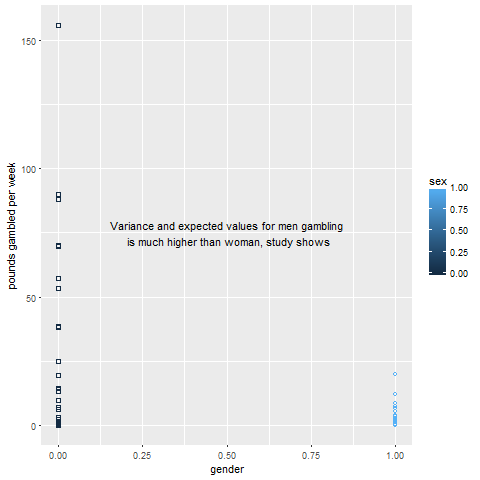
\includegraphics[width=15cm,height=15cm]{expenses.png}
	\caption[expenses]{plot of gambling amounts split by gender}
	\label{rVals}
\end{figure}

\item  Finish R exercises 1,2,4,6 on page 30-31 of the textbook.  (exercises from chapter 2).  Submit your answers for {\color{red}ALL} questions.\\
1
\begin{enumerate}

	\item 
		\begin{verbatim}
	> lTG<-lm(gamble ~ sex + status + income + verbal, teengamb)
	> summary(lTG)
	
	Call:
	lm(formula = gamble ~ sex + status + income + verbal, data = teengamb)
	
	Residuals:
	Min      1Q  Median      3Q     Max 
	-51.082 -11.320  -1.451   9.452  94.252 
	
	Coefficients:
	Estimate Std. Error t value Pr(>|t|)    
	(Intercept)  22.55565   17.19680   1.312   0.1968    
	sex         -22.11833    8.21111  -2.694   0.0101 *  
	status        0.05223    0.28111   0.186   0.8535    
	income        4.96198    1.02539   4.839 1.79e-05 ***
	verbal       -2.95949    2.17215  -1.362   0.1803    
	---
	Signif. codes:  0 ‘***’ 0.001 ‘**’ 0.01 ‘*’ 0.05 ‘.’ 0.1 ‘ ’ 1
	
	Residual standard error: 22.69 on 42 degrees of freedom
	Multiple R-squared:  0.5267,	Adjusted R-squared:  0.4816 
	F-statistic: 11.69 on 4 and 42 DF,  p-value: 1.815e-06
	\end{verbatim}
	$R^2=.53$, so 53 percent of the model is explained by the predictors
	\item
	\begin{verbatim}
		> rTG = residuals(lTG)
		> mTG = max(rTG)
		> which(rTG==mTG)
		[1] 94.25222
		24 
	\end{verbatim} 
	Thus, case 24 has the highest residual with a residual of 94.252
	\item 
	\begin{verbatim}
		> weighted.mean(rTG)
		[1] -3.07083e-17
	\end{verbatim}mean ~ -3.07e-17, median = -1.451
	\item
	\begin{verbatim}
		> var(rTG,fTG)
		[1] -5.309559e-14
	\end{verbatim} 
	$\Cov(\text{Residuals,Fitted Values}) = -5.3096$e-14
	\item 
	\begin{verbatim}
		> var(rTG,teengamb$income)
		[1] -5.576533e-15
	\end{verbatim}
	$\Cov(\text{Residuals,income}) = -5.577$e-15
	\item 
	\begin{verbatim}
		> print(mmean-fmean)
		[1] 25.90921
	\end{verbatim}
	MaleMean - FemaleMean = 25.90921 pounds
\end{enumerate}
2
\begin{enumerate}
	
	\item 
	\begin{verbatim}
		> usModel <- lm(wage~educ+exper,uswages)
		> usLModel <- lm(log(wage)~educ+exper,uswages)
		> summary(usModel)
		
		Call:
		lm(formula = wage ~ educ + exper, data = uswages)
		
		Residuals:
		Min      1Q  Median      3Q     Max 
		-1018.2  -237.9   -50.9   149.9  7228.6 
		
		Coefficients:
		Estimate Std. Error t value Pr(>|t|)    
		(Intercept) -242.7994    50.6816  -4.791 1.78e-06 ***
		educ          51.1753     3.3419  15.313  < 2e-16 ***
		exper          9.7748     0.7506  13.023  < 2e-16 ***
		---
		Signif. codes:  0 ‘***’ 0.001 ‘**’ 0.01 ‘*’ 0.05 ‘.’ 0.1 ‘ ’ 1
		
		Residual standard error: 427.9 on 1997 degrees of freedom
		Multiple R-squared:  0.1351,	Adjusted R-squared:  0.1343 
		F-statistic:   156 on 2 and 1997 DF,  p-value: < 2.2e-16
		
		> summary(usLModel)
		
		Call:
		lm(formula = log(wage) ~ educ + exper, data = uswages)
		
		Residuals:
		Min      1Q  Median      3Q     Max 
		-2.7533 -0.3495  0.1068  0.4381  3.5699 
		
		Coefficients:
		Estimate Std. Error t value Pr(>|t|)    
		(Intercept) 4.650319   0.078354   59.35   <2e-16 ***
		educ        0.090506   0.005167   17.52   <2e-16 ***
		exper       0.018079   0.001160   15.58   <2e-16 ***
		---
		Signif. codes:  0 ‘***’ 0.001 ‘**’ 0.01 ‘*’ 0.05 ‘.’ 0.1 ‘ ’ 1
		
		Residual standard error: 0.6615 on 1997 degrees of freedom
		Multiple R-squared:  0.1749,	Adjusted R-squared:  0.174 
		F-statistic: 211.6 on 2 and 1997 DF,  p-value: < 2.2e-16
	\end{verbatim}The t value is quite high for the education coefficient and thus we can trust it. Since the coefficient is at 51.17 approximately we can say that for every year of education they make, they get a boost, on average, of 51.17 dollars per week.
	\item If we take the log of weekly wages, we have a much reduced weekly wage for each case. Thus, the coefficient, now measured at approximately 0.091 is the additional logged pay per week added per year of education
\end{enumerate}
4
\item
\begin{verbatim}
	> prostateModel = lm(lpsa~lcavol,prostate)
	> tempS=summary(prostateModel)
	> rVals = double()
	> rSE = double()
	> for( nam in vars)
	+ {
	+   prostateModel = update(prostateModel, as.formula(paste('~ . +', nam)))
	+   tempS = (summary(prostateModel))
	+   print(tempS$r.squared)
	+   rVals=append(rVals, c(tempS$r.squared))
	+   rSE=append(rSE,tempS$sigma)
	+   
	+ }
	[1] 0.5394319
	[1] 0.5859345
	[1] 0.5892177
	[1] 0.597575
	[1] 0.6441024
	[1] 0.645113
	[1] 0.650644
	[1] 0.6547541
	[1] 0.6547541
	Warning messages:
	1: In model.matrix.default(mt, mf, contrasts) :
	the response appeared on the right-hand side and was dropped
	2: In model.matrix.default(mt, mf, contrasts) :
	problem with term 9 in model.matrix: no columns are assigned
	> #need to remove the last elements
	> rVals = head(rVals,-1)
	> rSE = head(rSE,-1)
	> png("C:/Users/alexander/Documents/GitHub/regressions/rVals.png")
	> qplot(1:8,rVals)
	> dev.off()
	> png("C:/Users/alexander/Documents/GitHub/regressions/rSE.png")
	> qplot(1:8,rSE)
	> dev.off()
	null device 
	1 
\end{verbatim}
\begin{figure}[H]
	\centering
	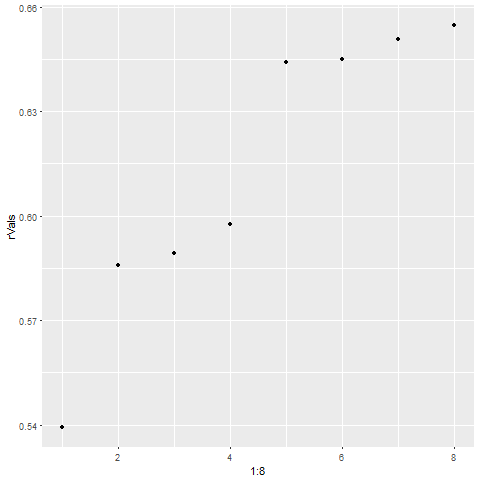
\includegraphics[width=15cm,height=15cm]{rVals.png}
	\caption[rVals]{R squared value over each element being added}
	\label{rVals}
\end{figure}
\item
\begin{figure}[H]
	\centering
	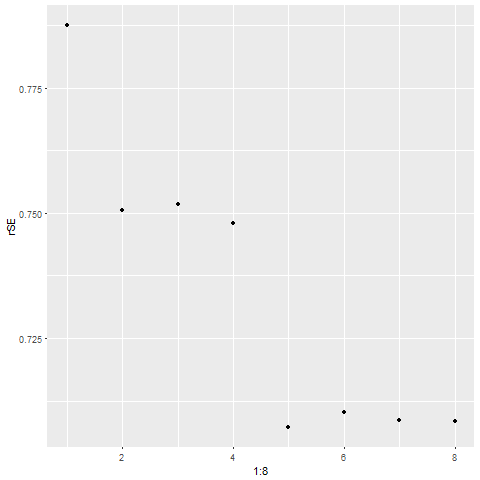
\includegraphics[width=15cm,height=15cm]{rSE.png}
	\caption[rSE]{residual squared error}
	\label{residual squared errors}
\end{figure}

6
\begin{enumerate}
	\item 
	\begin{verbatim}
		> cheeseModel = lm(taste~Acetic + H2S + Lactic, cheddar)
		> summary(cheeseModel)
		
		Call:
		lm(formula = taste ~ Acetic + H2S + Lactic, data = cheddar)
		
		Residuals:
		Min      1Q  Median      3Q     Max 
		-17.390  -6.612  -1.009   4.908  25.449 
		
		Coefficients:
		Estimate Std. Error t value Pr(>|t|)   
		(Intercept) -28.8768    19.7354  -1.463  0.15540   
		Acetic        0.3277     4.4598   0.073  0.94198   
		H2S           3.9118     1.2484   3.133  0.00425 **
		Lactic       19.6705     8.6291   2.280  0.03108 * 
		---
		Signif. codes:  0 ‘***’ 0.001 ‘**’ 0.01 ‘*’ 0.05 ‘.’ 0.1 ‘ ’ 1
		
		Residual standard error: 10.13 on 26 degrees of freedom
		Multiple R-squared:  0.6518,	Adjusted R-squared:  0.6116 
		F-statistic: 16.22 on 3 and 26 DF,  p-value: 3.81e-06
	\end{verbatim}
	intercept -29, acetic 0.3277, H2S 3.9, Lactic 19.7
	\item 
	\begin{verbatim}
		> cheeseFit = fitted(cheeseModel)
		> actual = cheddar$taste
		> corrCheese = cor(actual,cheeseFit)
		> print(corrCheese^2)
		[1] 0.6517747
	\end{verbatim}
	we get a value of .6518 which is the multiple R Squared found in the summary
	\item
	\begin{verbatim}
		> cheeseModelNoInt = lm(taste~Acetic + H2S + Lactic+0, cheddar)
		> summary(cheeseModelNoInt)
		
		Call:
		lm(formula = taste ~ Acetic + H2S + Lactic + 0, data = cheddar)
		
		Residuals:
		Min       1Q   Median       3Q      Max 
		-15.4521  -6.5262  -0.6388   4.6811  28.4744 
		
		Coefficients:
		Estimate Std. Error t value Pr(>|t|)    
		Acetic   -5.454      2.111  -2.583  0.01553 *  
		H2S       4.576      1.187   3.854  0.00065 ***
		Lactic   19.127      8.801   2.173  0.03871 *  
		---
		Signif. codes:  0 ‘***’ 0.001 ‘**’ 0.01 ‘*’ 0.05 ‘.’ 0.1 ‘ ’ 1
		
		Residual standard error: 10.34 on 27 degrees of freedom
		Multiple R-squared:  0.8877,	Adjusted R-squared:  0.8752 
		F-statistic: 71.15 on 3 and 27 DF,  p-value: 6.099e-13
		
		> CF = fitted(cheeseModelNoInt)
		> print(cor(actual,CF)^2)
		[1] 0.6244075 	
	\end{verbatim}
	 R squared is now .8877, much higher than the previous version, using corr squared we get .6244 which makes more sense
	\item        
	\begin{verbatim}
		> qrc = qr(cheeseModel)
		> qrCC = t(qr.Q(qrc)) %*% actual
		> backsolve(qr.R(qrc),qrCC)
		[,1]
		[1,] -28.8767696
		[2,]   0.3277413
		[3,]   3.9118411
		[4,]  19.6705434
	\end{verbatim}    

\end{enumerate}
\end{enumerate}

\end{document}
